\documentclass[12pt]{article}
\usepackage[margin=1.0in]{geometry}
\usepackage{amsmath}
\usepackage{amssymb}
\usepackage{amsfonts}
\usepackage{parskip}
\usepackage{natbib}
% \usepackage{color}
% \usepackage[dvipsnames]{xcolor}
\usepackage{caption}
%\usepackage{tabularx, booktabs}
%\usepackage{float}
\usepackage{adjustbox}
\usepackage[toc,page]{appendix}
\usepackage{enumitem}
\usepackage{multirow}
\usepackage{setspace}
\usepackage{url}
\usepackage{xr}

\externaldocument[S-]{Supplement}

\doublespacing

\newif\ifdic   % Type \ifdic at the beginning of any optional section... use \fi to denote the end of the optional section
  % See: http://tex.stackexchange.com/questions/33576/conditional-typesetting-build
%\dictrue         % comment out if I want to hide DIC and model fit paragraphs

% \newcommand{\adam}[1]{{\color{blue} ADAM: #1}}
% \newcommand{\jarad}[1]{{\color{Orange} JARAD: #1}}

\newenvironment{indpar}[1]%
     {\begin{list}{}%
             {\setlength{\leftmargin}{#1}}%
             \item[]%
     }
     {\end{list}}

\newcommand{\vn}{\textbf{n}}
\newcommand{\vp}{\textbf{p}}
\newcommand{\vX}{\textbf{X}}
\newcommand{\vZ}{\textbf{Z}}
\newcommand{\vbeta}{\boldsymbol{\beta}}
\newcommand{\vxi}{\boldsymbol{\xi}}

\newcommand{\Exp}{\mbox{Exp}}
\newcommand{\Ga}{\mbox{Ga}}
\newcommand{\We}{\mbox{We}}
\newcommand{\LN}{\mbox{LN}}
\newcommand{\Po}{\mbox{Po}}
\newcommand{\Mult}{\mbox{Mult}}

\newcommand{\pdet}{p^{(det)}}
\newcommand{\ind}{\stackrel{ind}{\sim}}
\newcommand{\Fm}{F_T^{(M)}}

\providecommand{\blind}{0}

\title{Assessing the impacts of time to detection distribution assumptions on detection probability estimation}

\if0\blind
\author{Adam Martin-Schwarze, Jarad Niemi, and Philip Dixon\\
Department of Statistics, Iowa State University, Ames, Iowa}
\fi

\begin{document}

\maketitle
\newpage

%\tableofcontents 

\begin{abstract}

Abundance estimates from animal point-count surveys require accurate estimates of detection probabilities.  
The standard model for estimating detection from removal-sampled point-count surveys assumes that organisms at a survey site are detected at a constant rate; however, this assumption is often not justified.  
%Detection rates can be influenced by organismal behaviors, survey methodology, and observer effort.  
%Failure to account for non-constant detection leads to biased estimates of detection and therefore of abundance.  
We consider a class of N-mixture models that allows for detection heterogeneity over time through a flexibly defined time-to-detection distribution (TTDD) and allows for fixed and random effects for both abundance and detection.
%We consider a class of N-mixture models that allow for detection heterogeniety through a mixture component, flexible two-parameter time-to-detection distributions (TTDDs), and allows for fixed and random effects for both abundance and detection.
%Whereas, under the standard approach, detection probability is modeled by dividing the observation period into equal-duration intervals, we instead model the detection {\it rate} in continuous time via a time-to-detection distribution (TTDD) embedded within a hierarchical N-mixture framework.  
Our model is thus a combination of survival time-to-event analysis with unknown-N, unknown-p abundance estimation.  
We specifically explore two-parameter families of TTDDs, e.g. gamma, that can additionally include a mixture component to model increased probability of detection in the initial observation period.
We find that modeling a TTDD by using a mixture component is necessary when data have a chance of arising from a distribution of this nature.
In addition, two-parameter distributions can outperform exponential-based models both when the truth is exponential or non-exponential.
Finally, we analyze an Overbird data set from the Chippewa National Forest using mixed effect models for both abundance and detection.
We demonstrate that the effects of explanatory variables on abundance and detection are consistent across mixture TTDDs but that flexible TTDDs result in lower estimated probabilities of detection and therefore higher estimates of abundance. 
%We find that modeling a TTDD by using a mixture component for increased probability of detection in the initial observation period is necessary when data have a chance of arising from distributions of this nature.
%In addition, the flexibility offered by two-parameter distributions, e.g. gamma, can outperform exponential based models when the truth is exponential or non-exponential.
%Finally, we analyze an Overbird data set from the Chippewa National Forest using mixed effect models for both abundance and detection and demonstrate that the effects of explanatory variables on abundance and detection are consistent across mixture TTDDs and that flexible TTDDs result in lower estimated probabilities of detection and therefore higher estimates of abundance. 
% We apply this model to Ovenbird counts from the Chippewa National Forest and to datasets simulated under different time-to-detection patterns.  
% Models assuming constant detection rates produce biased estimates of detection when true detection rates vary with time, whereas models allowing for variable detection (assuming gamma, Weibull, or lognormal distributed times to detection) produce less biased estimates of the detection probability and nominal credible interval coverage.  
% Models ignoring detection heterogeneity across subgroups yield biased estimates of detection when such heterogeneity exists, whereas models accounting for detection heterogeneity (modeled as a mixture) return reasonable coverage rates and can outperform heterogeneity-ignorant models even when there is no heterogeneity.

{\bf Keywords:} abundance; availability; N-mixture model; point counts; removal sampling; survival analysis; Markov chain Monte Carlo; Stan

\end{abstract}

\newpage
\section{Introduction}\label{sec:intro}

Abundance estimates from animal point-count surveys require accurate estimates of detection probabilities.  
Removal sampling, where individuals are solely counted on their first capture, provides one established methodology for estimating detection probabilities \citep{Farnsworth2002}.
% cost-effective in that it requires neither multiple observers nor multiple site visits.
%Removal sampling is a species abundance surveying methodology in which observers capture and physically remove animals at a survey site over a series of trapping sessions.
%Assuming that individual capture rates remain constant over all trapping sessions, it is possible to estimate the proportion of individuals still not captured from the pattern of captures over time .  
%\citet{Farnsworth2002} adapted removal sampling to point-count surveys, suggesting that if: (i) observers record only the first time-to-detection for each animal, and (ii) times to first detection are interval-censored, then data will be similar in for to traditional removal sampled data.
%In the analysis of such data, the observation period is subdivided into unit intervals of equal duration, each of which is equivalent to a trapping session.
%Farnsworth's removal assumptions:\\
%(i) Closed population during survey\\
%(ii) no double-counting\\
%(iii) easy-to-detect group is entirely counted during first interval\\
%(iv) TTDD for hard-to-detect group is correct after the end of the observation period\\
%(v) if using limited radius counts, they are accurate
% Johnson2008: all birds present are available for detection
A typical assumption in removal sampling is a constant detection rate throughout the observation period, but this assumption is often unjustified \citep{Alldredge2007}.  
In particular, animal behaviors such as intermittent singing in birds and frogs or diving in whales \citep{Scott2005, Diefenbach2007, Reidy2011}, differences in behavior across subgroups of animals \citep{Otis1978, Farnsworth2005}, observer impacts on animal behaviors \citep{McSheaRappole1997, Rosenstock2002, Alldredge2007}, and variations in observer effort, e.g. saturation or lack of settling in period \citep{Petit1995, LeeMarsden2008, Johnson2008}, can all lead to time-varying rates of detection.

In this manuscript, we develop a model for scenarios where detection rates are not constant over time. 
We consider the first time-to-detection as is done in survival analysis, defining a continuous random variable $T$ for each individual's time to first detection with a probability density function (pdf) $f_T(t)$ and cumulative distribution function (cdf) $F_T(t)$.  
We refer to the distribution of $T$ as a time-to-detection distribution (TTDD).  
One common strategy to deal with data that do not fit a constant-detection assumption is to model increased detection probability in the initial observation period via a mixture component \citep{Farnsworth2002, Farnsworth2005, EffordDawson2009, Etterson2009, Reidy2011}, although this is not yet the standard \citep{Solymos2013, Amundson2014, Reidy2016}. 
We consider the choice of whether to include a mixture component in conjunction with TTDDs with non-constant rates.

Unlike most survival analyses, the number of individuals $N$ present at a survey is unknown and may be the primary quantity of interest.  
We embed the TTDD in a hierarchical framework for multinomial counts using an N-mixture model \citep{Wyatt2002, Royle2004NMixture}.  
For our purposes, the N-mixture framework provides three clear benefits: 1) its multinomial data framework accords with the interval-censored data collection that is customary in point-count surveys \citep{Ralph1995}, 2) the hierarchical structure readily lends itself to including abundance- and detection-related covariates and random effects \citep{Dorazio2005, Etterson2009, Amundson2014}, and 3) for a Bayesian analysis, we can sample the posterior joint distribution of N-mixture parameters straight-forwardly using Markov chain Monte Carlo (MCMC).  
The N-mixture framework models abundance as a latent variable with a Poisson or other discrete distribution and independently models detection probabilities.  
Several previous studies have employed the N-mixture framework to analyze removal sampled point-count data while assuming constant detection rates \citep{Royle2004Generalized, Dorazio2005, Etterson2009, Solymos2013, Amundson2014, Reidy2016}.  



%Application of this methodology generally assumes that organisms at a survey site are detected at a constant rate \citep{Farnsworth2005, Etterson2009, Solymos2013, Amundson2014, Reidy2016}; however, this assumption is often not justified in the field.  
%Failure to account for non-constant detection leads to biased estimates of detection and therefore of abundance.  



Framing a model in terms of time-to-detection leads to two practical differences vis-a-vis constant-detection models.  
First, in order to model covariate and random effects on detection, we perform mixed effects linear regression on the log of the rate parameter as in \citet{Solymos2013}, whereas most existing studies instead construct regression models on the logit of the equal-interval detection probability.  
The latter is not possible when detection rates are not constant.  
Second, because we can obtain interval-specific detection probabilities from the TTDD by partitioning its cdf, we can directly model the data according to their existing interval structure rather than subdividing the observation period into intervals of equal duration.  
Indeed our model fits exact time-to-detection data, whereas existing constant-detection removal models only approximate exact data by subdividing the observation interval into a large number of fine equal-duration intervals \citep{Reidy2011, Amundson2014}.


% \adam{Based on further lit review, I think I need to insert a paragraph here about what time-varying modeling has been done.  
% In the fisheries world, models of time-varying catchability have been implemented -- see Schnute 1983, Scruton and Gibson (ref: Mantyniemi), and Mantyniemi2015 for examples.  
% Also, Alldredge 2007 implements a complete-history of detection model (technically mark-recapture, not removal) that estimates interval-specific detection probabilities (complete with covariates and detection heterogeneity).  
% However, it cannot be applied in a removal context, because removal data contains only first times to detection, and the Alldredge model requires subsequent observations -- removal models compensate by specifying a TTDD, thus enabling us to extrapolate beyond the observation period.}  

Section \ref{sec:data} provides a description of the interval-censored time-to-detection avian point count data under consideration.
Section \ref{sec:model} introduces an N-mixture model with a generically defined TTDD for estimating abundance from removal-sampled point-count surveys.
%In addition, we discuss reasonable default priors and MCMC analysis used to estimate parameters in these models.
Section \ref{sec:sim} provides three simulation studies to assess the impact of TTDD choice on estimated detection probability. 
Section \ref{sec:ovenbirds} analyzes an Ovenbird data set under different TTDDs to determine the impact of this choice on estimated detection probability and therefore estimated abundance.

\section{Interval-censored point counts}\label{sec:data}

Our analysis is motivated by avian point-count surveys in Chippewa National Forest from 2008-2013 as part of the Minnesota Forest Breeding Bird Project (MNFB) \citep{Hanowski1995}.  
%However, the model we describe is appropriate for point-count surveys of any species, so long as time-to-first-detection data are available.  
For our analysis, we focused on Ovenbird counts selected from one habitat type: sawtimber red pine stands with no recent logging activity.  
Each stand had up to four sites with sufficient geographical distance between sites to reduce or eliminate overlapping territories.
The data included 65 sites and a total of 381 surveys with site specific variables including site age,  stock density, and an indicator of select-/partial-cut logging during the 1990s. 

Single-visit (per year) point-count surveys were conducted by trained observers at each site once annually (weather permitting).  
Fourteen different observers conducted surveys during the study period and 69\% of surveys in our dataset involved observers in their first year at the MNFB.  
Survey durations were 10 minutes, with times to first detection censored into nine intervals: a two-minute interval followed by eight one-minute intervals.  
During each survey, the Julian date, time of day, and temperature were recorded. 

% A total of 947 Ovenbirds were counted with a maximum of eight birds counted in any single survey.  
% The counts of Ovenbirds by interval, across all sites, were 596, 69, 62, 68, 43, 33, 35, 27, and 14.

While we focus on the estimation of detection probability in avian populations, the approach we describe is appropriate for point-count surveys of any species.
The methodology allows the analysis of data with 1) recorded first (possible censored) detection of each individual, 2) site-specific explanatory variables, and 3) survey-specific explanatory variables.  






\section{Continuous time-to-detection N-mixture models} \label{sec:model}

Before considering interval censoring and explanatory variables, we first present the scenario of exact time to detections with no explanatory variables. 
We then incorporate interval censoring and follow with inclusion of fixed and random effects for abundance and detection. 

\subsection{Exact time to detection}

Suppose that, for each survey $s$ ($s=1,\dots,S$), $N_s$ individuals are present.  
Imagine an observer could remain at the survey location until every individual is detected, recording the time to detection $t_{sb}$ (for bird, $b=1,\dots,N_s$) for each.
Assuming detection times for all individuals at a survey are independent, identically distributed according to a common time-to-detection distribution (TTDD), we define $T_{sb}$ as a random variable with cumulative distribution function (cdf) $F_T(t)$ and probability density function (pdf) $f_T(t)$.
In reality, times to first detection are often truncated due to a finite survey length of $C$, meaning that each individual has a detection probability $\pdet=F_T(C)$.  
The conditional distribution of observed detection times then has pdf $f_{T|det}(t)= f_T(t)/F_T(C)$ for $0<t<C$, cdf $F_{T|det}(t) = \int_0^t f_{T|det}(x) dx$, and instantaneous detection rate, or hazard function, is $h(t) = f_T(t) / [1-F_T(t)]$. 
We model the number of individuals at survey $s$ for which $t_{sb}$ is actually observed as $n_{s}^{(obs)} \ind \mbox{Binomial}\left(N_{s}, \pdet\right)$. 
%$T_{sb|det} \ind f_{T|det}(t_{sb})$ where $T_{sb|det}$ is observed only for those $n_s^{(obs)}$ individuals whose observed time to first detection is less than $C$, i.e. $t_{sb}<C$. 

A common choice for TTDD is an exponential distribution, i.e. $T_{sb}\ind \mbox{Exp}(\varphi)$, which imposes a constant first detection rate, i.e. $h(t) = \varphi$.
Choosing another TTDD can allow for a systematic non-constant detection regime. 
For example, to model an observer effect where: (i) the observer's arrival suppresses or stimulates detectable cues, but (ii) organisms acclimate and gradually return to constant detection, a gamma TTDD could be appropriate.
In addition to an exponential and gamma TTDD, we also consider Weibull and lognormal as these distributions are often used in survival analysis. 
To facilitate the later inclusion of fixed and random effects, we use the following rate-based parameterizations: $T\sim \Exp(\varphi), E[T]=1/\varphi$; $T\sim \Ga(\alpha,\varphi), E[T] = \alpha/\varphi$; $T\sim \We(\alpha,\varphi), E[T]=\mathrm{\Gamma}(1+1/\alpha)/\varphi$; and $T\sim \LN(\varphi,\alpha), E[T] = e^{\alpha/2}/\varphi$.  
This parameterization of the lognormal relates to the standard ($\mu, \sigma^2$) parameterization by $\varphi = \exp(-\mu)$ and $\alpha = \sigma^2$.  %$\mu = -\log(\varphi)$
The exponential distribution is a special case of both the gamma and Weibull distributions when $\alpha=1$. 

Using maximum likelihood, we can estimate the parameters in a TTDD from exact times to first detection and thus estimate $\pdet$ and its uncertainty.
With an estimate and uncertainty for $\pdet$, we are in a scenario of a binomial model with unknown $N_s$ and ``known'' $p$ and thus can estimate $N_s$.
In these models, point estimates of $N_s$ are unstable unless $\pdet>0.4$ \citep{Olkin1981}.
One approach to regularizing these estimates is to construct a hierarchical model for the site-specific abundance, e.g. $N_s\ind \Po(\lambda)$ \citep{Raftery1988, Royle2004NMixture}. 
With this assumption, we can decompose $N_{s}$ into observed and unobserved portions: $n^{(obs)} \sim Po(\lambda \pdet)$ and, independently, $n_{s}^{(unobs)} \sim \Po\left(\lambda[1-\pdet]\right)$.
Although alternative distributions could be considered, e.g. negative binomial, our experience with Ovenbird point counts suggests that, after accounting for appropriate explanatory variables, the resulting abundances are likely underdispersed rather than overdispersed, and thus we will use the Poisson assumption here. 


\subsection{Interval-censored times to detection} \label{s:interval}

Due to the harried process of avian point counts, times to first detection are typically not recorded exactly, but are instead censored into $I$ intervals. 
Let $C_i$ for $i=1,\dots,I$ indicate the right endpoint of the $i$th interval then $C_I$ is the total survey duration and, letting $C_0=0$, the $i$th interval is $(C_{i-1},C_{i}]$. 
Let $n_{si}$ be the number of individuals counted during interval $i$ on survey $s$, $n_{s}^{(obs)} = \sum_{i=1}^I n_{si}$, and $\vn_{s}=(n_{s1},\dots,n_{sI})$.
Assuming independence amongst individuals and sites, we have $\vn_{s} \ind \Mult \left(n_{s}^{(obs)}, \vp_{s}\right)$, where $\vp_{s}=(p_{s1},\dots,p_{sI})$ and is calculated from the TTDD: $p_{si} = F_{T|det}(C_i) - F_{T|det}(C_{i-1})$.  

\subsection{Detection heterogeneity across subgroups} \label{s:subgroups}

It is common in avian point counts to observe increased detections in the first interval relative to an exponential distribution.
This is often understood to reflect unmodeled detection heterogeneity across behavioral groups in the study population.
Failure to account for such heterogeneity in the constant-detection scenario leads to negative bias in abundance estimates \citep{Otis1978}.
To accommodate this empirical observation, many models of interval-censored removal times define a TTDD with a mixture component to increase the probability of observing individuals in the first interval \citep{Farnsworth2002, Royle2004Generalized, Farnsworth2005, Alldredge2007, Etterson2009, Reidy2011}.
We specify a mixture TTDD with mixing parameter $\gamma\in[0,1]$, a point-mass during the first observation interval, and a continuous-time detection distribution $\Fm(t)$.  
The mixture TTDD cdf is defined: $F_T(t) = (1-\gamma) + \gamma \Fm(t)$ for $t>0$.
If $\gamma=1$, the non-mixture model is recovered.





\subsection{Incorporating explanatory variables}\label{sec:covariates}

As discussed in Section \ref{sec:data}, explanatory variables are available for sites and for surveys. 
Generally, we suspect that site variables, e.g. habitat, will affect abundance and survey variables, e.g. time of day, will affect detection probability. 
Thus, we allow for incorporating explanatory variables on both the abundance and detection.

To incorporate explanatory variables on abundance, we model the expected survey abundance $\lambda_{s}$ with log-linear mixed effects, i.e. $\log (\lambda_{s}) = \vX_{s}^A\vbeta^A + \vZ_{s}^A\vxi^A$ where $\vX_{s}^A$ are explanatory variables, $\vbeta^A$ is a vector of fixed effects, $\vZ_{s}^A$ specifies random effect levels, and $\xi_j^A \ind N(0,\sigma_{A[j]}^2)$ are random effects where $A[j]$ assigns the appropriate variance for the $j$th abundance random effect.  

To incorporate explanatory variables on detection probability, we let the continuous portion of the TTDD depend on the explanatory variables through the now site-specific parameter $\varphi_s$. 
Specifically, we model $\log(\varphi_{s}) = \vX_{s}^D\vbeta^D + \vZ_{s}^D\vxi^D$, where $\vX_{s}^D$ are explanatory variables, $\vbeta^D$ is a vector of fixed effects, $\vZ_{s}^D$ specifies random effect levels, $\xi_j^D \ind N(0,\sigma_{D[j]}^2)$ are random effects where $D[j]$ assigns the appropriate variance for the $j$th detection random effect.  
For simplicity, we assume the shape parameter $\alpha$ as constant across sites.



\subsection{Estimation}

For ease of reference, the final full model is provided in equation \eqref{eq:model} where the conditioning of the TTDD cdf on $\alpha$ and $\varphi_s$ is made explicit.
\begin{align}
n_s^{(obs)} &\ind \Po(\lambda_s \pdet_s) \nonumber\\
\vn_s &\ind \Mult(n_s^{(obs)}, \vp_s); \qquad \vp_s = (p_{s1},\dots,p_{sI}) \nonumber\\
\pdet_s &= F_T(C_I|\alpha,\varphi_s) \nonumber \\
p_{s1} &= \left[(1-\gamma) + \gamma\Fm(C_1|\alpha,\varphi_s)\right]/\pdet_s \label{eq:model} \\
p_{si} &= \gamma\left[\Fm(C_i|\alpha,\varphi_s) - \Fm(C_{i-1}|\alpha,\varphi_s)\right]/\pdet_s \nonumber\\
\log(\lambda_s) &= \vX_{s}^A\vbeta^A + \vZ_{s}^A\vxi^A; \qquad \xi_j^A \ind N(0,\sigma_{A[j]}^2) \nonumber\\
\log(\varphi_{s}) &= \vX_{s}^D\vbeta^D + \vZ_{s}^D\vxi^D; \qquad \xi_j^D \ind N(0,\sigma_{D[j]}^2) \nonumber
\end{align}
We adopt a Bayesian approach and therefore require a prior over the model parameters.
To ease construction of a default prior for this model, we standardize all explanatory variables and then construct priors to be diffuse within a reasonable range of values.
Normal prior mean and standard deviation (sd) for the abundance intercept was set at a median abundance of 3 birds per site and a 95\% probability of 0-14 birds present (counted and uncounted).  
Normal prior mean and sd for the detection intercept were chosen so that, based on an intercept-only non-mixture model with $\alpha=1$: (i) median prior detection probability was $p_{s}^{(det)} = 0.50$, and (ii) 95\% of the prior detection probability was within $p_{s}^{(det)} \in (0.01, 1.0)$.  
Normal priors for fixed effect parameters were centered at zero with standard deviations matching the appropriate intercept term.  
All standard deviations and $\alpha$ were given half-Cauchy priors with location 0 and scale 1 for the untruncated Cauchy, and the mixture parameter $\gamma$ was assigned a Unif(0,1) prior in mixture models.
All scalar parameters were assumed independent \emph{a priori}. 



We fit the models by MCMC sampling using the Bayesian statistical software Stan, implemented via the R package \texttt{rstan} version 2.8.0 \citep{Rstan2015}.  
Stan model code and \texttt{rstan} code to run the models can be found in the Supplementary Materials.  
We discarded half of the iterations as warmup and then thinned by 10.  
We monitored convergence of the MCMC chains using Geweke z-score diagnostics \citep{Geweke1991} and reran models if lack of convergence was indicated by a non-normal distribution of the z-scores or if the effective sample size for any parameter was below 1000.  
The number of iterations used depended on the model and is detailed later. 
For most models, we accepted Stan defaults for initial values; however, gamma and Weibull models sometimes failed to run unless care was taken in the specification of initial values.





%Thus, the link functions in our detection model are:
%\begin{alignat}{3}
%&\text{Exponential:\;} &&\log(\varphi_{s}) &&= \text{Intercept}^D + \vX_{s}^D\vbeta^D + \vZ_{s}^D\vxi^D = -\log(E[T_{sq}])\\
%&\text{Gamma:} &&\log(\varphi_{s}) &&= \text{Intercept}^D + \vX_{s}^D\vbeta^D + \vZ_{s}^D\vxi^D = -\log(E[T_{sq}]) + \log(\alpha)\\
%&\text{Weibull:}  &&\log(\varphi_{s}) &&= \text{Intercept}^D + \vX_{s}^D\vbeta^D + \vZ_{s}^D\vxi^D = -\log(E[T_{sq}]) + \log\left(\Gamma\left(1 + 1/k\right)\right)\\
%&\text{Lognormal:} &&-\mu_{s} &&= \text{Intercept}^D + \vX_{s}^D\vbeta^D + \vZ_{s}^D\vxi^D = -\log(E[T_{sq}]) + \sigma_{det}^2/2
%\end{alignat}

%\subsection{Abundance Model}


% We distinguish between non-constant detection and detection heterogeneity, which can be modeled in similar ways but refer to different mechanisms.  
% We reserve `detection heterogeneity' for differences across population subgroups.  
% It is often modeled using a mixture of detection distributions.  
% \citet{Farnsworth2002} introduce a finite-mixture for detection probabilities distinguishing between easy-to-detect individuals, which are always detected in first observation interval, and hard-to-detect individuals, which are detected at a constant rate.  
%  Heterogeneity at the individual level can be modeled as random effects in the calculation of detection probabilities \citep{DorazioRoyle2003, Mantyniemi2005}.  
% We use `non-constant detection' when detection rates for an organism change with time.  
% Models constructed to address detection heterogeneity may provide reasonable estimates for non-constant detection scenarios and vice versa \citep{Mantyniemi2005}.

%\adam{Individual effects on detection might suffer from identifiability issues. This was the subject of a dust-up between Pledger and Dorazio/Royle from 2003-2005.}




\ifdic\
\subsection{Model diagnostics}

To assess goodness of fit, we relied on posterior predictive checks \citep{Gelman1996}.  
%Posterior predictive checks assess whether a fitted model can effectively replicate datasets that look like the original data in key aspects, which are measured by check statistics.  
In particular, we are concerned with the goodness of fit for the TTDD distribution, so we defined a check statistic for each observation interval:
\[D(n_i) = \sum\limits_{s} n_{si} \big/ \sum\limits_{si} n_{si}\]
which is the proportion of the total count that occurs during interval $i$ marginally across all surveys.  
The posterior predictive p-value associated with each $D(n_i)$ is the proportion of replicate check statistics that have a larger value than the check statistic for the actual data.  
Posterior predictive p-values near to 0 or 1 are potentially indicators of a misspecified model.
We simulated replicate datasets and calculated the check statistic at each iteration of our MCMC sampling.  

We focus inference on the overall detection probability across all surveys: $\pdet = \sum\limits_{s}n_{s}^{(obs)}\big/$ $\sum\limits_{s}N_{s}$.  
Within simulation studies, we compared model estimates to true $\pdet$ values by percent coverage and by posterior p-values --- the proportion of MCMC samples having a smaller value than the true value.  

We compared different models by means of their goodness of fit and deviance information criterion (DIC) \citep{Spiegelhalter2002}.  
For the full model with random effects (Ovenbirds and Sim3), which is a missing data model, we used formulation DIC$_7$ from \citet{Celeux2006} for its ease of computation, but we acknowledge that it suffers some difficulties \citep{Celeux2006, Li2014}.
\fi




\section{Simulation studies} \label{sec:sim}

We conducted three simulation studies to explore the behavior of models with non-constant TTDDs.
The first study compares mixture vs non-mixture models.
The second study compares the TTDD families.
In the first two studies, we utilized intercept only models to focus attention on the TTDD. 
For the third study, we included fixed and random effects for both abundance and detection and again compared the distribution families. 
In all simulation studies, we focus on accuracy in estimation of $\pdet$ which then translates into estimation of abundance. 
For the following analyses we distinguish two categories of purely continuous TTDDs: peaked and nonpeaked.  
A peaked TTDD has a mode greater than zero (or $C_1$ for lognormal) while a non-peaked TTDD has a mode of zero (or less than $C_1$).









\subsection{Mixture versus non-mixture TTDDs}\label{sec:mixture}

To assess the need for incorporating a mixture component to increase the probability of detection in the initial interval as discussed in Section \ref{s:interval}, we simulated 16 intercept-only datasets from each of 14 TTDDs: each combination of peaked/non-peaked, mixture/non-mixture, and exponential/gamma/Weibull/lognormal, where all exponential models are non-peaked.  
We chose the number of surveys (381) and true parameter values (Table \ref{S-simvals}) to mimic values from the Ovenbird analysis (Section \ref{sec:ovenbirds}).  
In particular, we set parameters such that (i) the overall expected detection probability was 0.80, (ii) for mixture datasets, $\gamma = 0.65$ (meaning 35\% of individuals were immediately detected), (iii) in nonpeaked models, 70\% of \textit{detected} individuals were observed during the first two minutes, and (iv) in peaked models, the detection mode for `hard to detect' individuals occured at 5 minutes.

Each dataset was fit with two models: mixture and non-mixture version of the distribution family, e.g. exponential, used to simulate the data.
For each dataset-analysis combination, we ran 60,000 iterations which showed no evidence of lack of convergence according to the Geweke diagnostic and reached over 1,000 effective samples for all parameters. 

We summarized the analysis by calculating the average, across the simulations, of the posterior median of $\pdet$ (Med. $p$), the average proportion of the posterior distribution of $\pdet$ larger than the truth (Q($p$)), and average coverage for 50\% and 90\% credible intervals. If the analyses are providing a reasonable estimate of $\pdet$, we would expect Med. $p$ to be around the true value of 0.8, Q($p$) to be around 0.5 indicating that half of the posterior is above and below the true value of 0.8, and the coverage to be close to their credibility. Table \ref{tbl:sim1} provides a summary of these quantities. 
When a mixture model is used to simulate the data (bottom half of the table), there is clearly a benefit to using a mixture model for inference.  
Using a non-mixture model for inference, the credible interval coverage is near zero for most models with the exponential model overestimating $\pdet$ (Q($p$) $\approx 1$) and the other models underestimating. 
When a non-mixture model is used to simulate the data (top half of the table), there are no clearly discernable differences between the ability of a non-mixture or mixture model to capture $\pdet$. 
For nonpeaked non-mixture data (top 4 lines), the mixture model is less biased for lognormal and Weibull scenarios (Q($p$)$\approx 0.5$), and CIs are 15-40\% narrower (results not shown).
These results support the general default use of a mixture model over a non-mixture model.

\ifdic
\begin{table}[ht]\centering\small
\begin{tabular}{l|l|l|l|cccc|cccc||r}
 \multicolumn{4}{c|}{ } & \multicolumn{4}{c|}{\underline{Non-mixture model}} & \multicolumn{4}{c||}{\underline{Mixture model}} & \\
 \multicolumn{4}{c|}{ } & Med. $p$ & Q($p$) & 50\% & 90\% & Med. $p$ & Q($p$) & 50\% & 90\% & $\Delta$ DIC \\ 
  \hline
  \hline
 \parbox[t]{2mm}{\multirow{14}{*}{\rotatebox[origin=c]{90}{TTDD used to simulate data}}} & \parbox[t]{2mm}{\multirow{7}{*}{\rotatebox[origin=c]{90}{Non-mixture}}} & \parbox[t]{2mm}{\multirow{3}{*}{\rotatebox[origin=c]{90}{Nonpk.}}} & Gamma & 0.76 & 0.41 & 0.75 & 0.88 & 0.84 & 0.66 & 0.56 & 0.94 & 0.24 \\ 
 & & &   Lognormal & 0.66 & 0.17 & 0.31 & 0.62 & 0.78 & 0.48 & 0.62 & 1.00 & -0.67 \\ 
 & & &   Weibull & 0.69 & 0.25 & 0.38 & 0.75 & 0.79 & 0.51 & 0.75 & 1.00 & 0.37 \\ 
  \cline{3-13}
 & & &   Exponential & 0.80 & 0.54 & 0.44 & 0.94 & 0.79 & 0.38 & 0.31 & 0.88 & 1.48 \\ 
  \cline{3-13}
 & & \parbox[t]{2mm}{\multirow{3}{*}{\rotatebox[origin=c]{90}{Peaked}}} &  Gamma & 0.80 & 0.55 & 0.50 & 1.00 & 0.82 & 0.70 & 0.38 & 0.88 & 0.96 \\ 
 & & &   Lognormal & 0.78 & 0.31 & 0.50 & 0.94 & 0.80 & 0.48 & 0.62 & 1.00 & 0.97 \\ 
 & & &   Weibull & 0.79 & 0.49 & 0.56 & 0.94 & 0.82 & 0.66 & 0.44 & 0.88 & 1.28 \\ 
  \cline{2-13}
& \parbox[t]{2mm}{\multirow{7}{*}{\rotatebox[origin=c]{90}{Mixture}}} & \parbox[t]{2mm}{\multirow{3}{*}{\rotatebox[origin=c]{90}{Nonpk.}}} & Gamma & 0.67 & 0.17 & 0.12 & 0.81 & 0.76 & 0.41 & 0.69 & 1.00 & 0.51 \\ 
 & & &   Lognormal & 0.56 & 0.04 & 0.00 & 0.31 & 0.72 & 0.30 & 0.44 & 0.88 & 0.33 \\ 
 & & &   Weibull & 0.51 & 0.02 & 0.00 & 0.06 & 0.71 & 0.32 & 0.44 & 1.00 & 2.40 \\ 
  \cline{3-13}
 & & &   Exponential & 0.96 & 1.00 & 0.00 & 0.00 & 0.77 & 0.37 & 0.38 & 0.94 & 122.81 \\ 
  \cline{3-13}
 & & \parbox[t]{2mm}{\multirow{3}{*}{\rotatebox[origin=c]{90}{Peaked}}} & Gamma & 0.28 & 0.00 & 0.00 & 0.00 & 0.74 & 0.33 & 0.31 & 0.88 & 31.84 \\ 
 & & &   Lognormal & 0.22 & 0.00 & 0.00 & 0.00 & 0.76 & 0.36 & 0.38 & 0.94 & 63.65 \\ 
 & & &   Weibull & 0.22 & 0.00 & 0.00 & 0.00 & 0.70 & 0.29 & 0.56 & 0.94 & 28.30 \\ 
   \hline
\end{tabular}
\caption{Summary of mixture vs. non-mixture model fits.  
In all cases, the inference model family matches the dataset family.  
Med $p$: average across simulations of the posterior median of $\pdet$ (true value = 0.80).  
Q($p$): average proportion of the posterior distribution of $\pdet$ that is larger than the true value.  
50\% and 90\% coverage is expressed as the proportion of 16 simulations for which the true value of $\pdet$ lies within the appropriate credible interval.  
$\Delta$ DIC: mean difference in DIC between the incorrect-mixture model minus the true model.
}
\label{tbl:sim1}
\end{table}

\else

\begin{table}[ht]\centering\small
\begin{tabular}{l|l|l|l|cccc|cccc}
 \multicolumn{4}{c|}{ } & \multicolumn{4}{c|}{\underline{Non-mixture model}} & \multicolumn{4}{c}{\underline{Mixture model}} \\
 \multicolumn{4}{c|}{ } & Med. $p$ & Q($p$) & 50\% & 90\% & Med. $p$ & Q($p$) & 50\% & 90\% \\ 
  \hline
  \hline
 \parbox[t]{2mm}{\multirow{14}{*}{\rotatebox[origin=c]{90}{TTDD used to simulate data}}} & \parbox[t]{2mm}{\multirow{7}{*}{\rotatebox[origin=c]{90}{Non-mixture}}} & \parbox[t]{2mm}{\multirow{3}{*}{\rotatebox[origin=c]{90}{Nonpk.}}} & Gamma & 0.76 & 0.41 & 0.75 & 0.88 & 0.84 & 0.66 & 0.56 & 0.94 \\ 
 & & &   Lognormal & 0.66 & 0.17 & 0.31 & 0.62 & 0.78 & 0.48 & 0.62 & 1.00  \\ 
 & & &   Weibull & 0.69 & 0.25 & 0.38 & 0.75 & 0.79 & 0.51 & 0.75 & 1.00 \\ 
  \cline{3-12}
 & & &   Exponential & 0.80 & 0.54 & 0.44 & 0.94 & 0.79 & 0.38 & 0.31 & 0.88  \\ 
  \cline{3-12}
 & & \parbox[t]{2mm}{\multirow{3}{*}{\rotatebox[origin=c]{90}{Peaked}}} &  Gamma & 0.80 & 0.55 & 0.50 & 1.00 & 0.82 & 0.70 & 0.38 & 0.88 \\ 
 & & &   Lognormal & 0.78 & 0.31 & 0.50 & 0.94 & 0.80 & 0.48 & 0.62 & 1.00 \\ 
 & & &   Weibull & 0.79 & 0.49 & 0.56 & 0.94 & 0.82 & 0.66 & 0.44 & 0.88 \\ 
  \cline{2-12}
& \parbox[t]{2mm}{\multirow{7}{*}{\rotatebox[origin=c]{90}{Mixture}}} & \parbox[t]{2mm}{\multirow{3}{*}{\rotatebox[origin=c]{90}{Nonpk.}}} & Gamma & 0.67 & 0.17 & 0.12 & 0.81 & 0.76 & 0.41 & 0.69 & 1.00 \\ 
 & & &   Lognormal & 0.56 & 0.04 & 0.00 & 0.31 & 0.72 & 0.30 & 0.44 & 0.88 \\ 
 & & &   Weibull & 0.51 & 0.02 & 0.00 & 0.06 & 0.71 & 0.32 & 0.44 & 1.00 \\ 
  \cline{3-12}
 & & &   Exponential & 0.96 & 1.00 & 0.00 & 0.00 & 0.77 & 0.37 & 0.38 & 0.94 \\ 
  \cline{3-12}
 & & \parbox[t]{2mm}{\multirow{3}{*}{\rotatebox[origin=c]{90}{Peaked}}} & Gamma & 0.28 & 0.00 & 0.00 & 0.00 & 0.74 & 0.33 & 0.31 & 0.88 \\ 
 & & &   Lognormal & 0.22 & 0.00 & 0.00 & 0.00 & 0.76 & 0.36 & 0.38 & 0.94 \\ 
 & & &   Weibull & 0.22 & 0.00 & 0.00 & 0.00 & 0.70 & 0.29 & 0.56 & 0.94 \\ 
   \hline
\end{tabular}
\caption{Summary of mixture vs. non-mixture model fits.  
In all cases, the inference model family matches the dataset family.  
Med $p$: average across simulations of the posterior median of $\pdet$ (true value = 0.80).  
Q($p$): average proportion of the posterior distribution of $\pdet$ that is larger than the true value.  
50\% and 90\% coverage is expressed as the proportion of 16 simulations for which the true value of $\pdet$ lies within the appropriate credible interval.  
}
\label{tbl:sim1}
\end{table}
\fi




% Median posterior abundance from mixture models was unbiased for non-mixture data and positively biased by only 4-15\% for mixture data.  
% Median posterior abundance from non-mixture models applied to non-mixture data were unbiased (exponential and peaked) or biased by 5-24\% (nonpeaked); however, for mixture data, the non-mixture models were biased by 20-60\% (nonpeaked), -17\% (exponential), and 183-265\% (peaked).  
% For the time-varying distributions, non-mixture models not only had greater bias, but 95\% credible intervals were generally 10-40\% wider (470\% wider for peaked mixture data).
% For exponential datasets, the non-mixture model credible intervals were 28\% narrower for non-mixture data and an unrealistic 95\% narrower for mixture data.

% Possible other comments
%(1) For nonpeaked data, the true inference model is biased low\\
%(2) Mixture inference models generate higher estimates than non-mixture models\\
%(3) True models are generally good\\
%(4) Estimates of non-mixture peaked data are much more precise\\
%(5) Note that plots of TTDD at the median are indistinguishable from the truth except in the blatant fail scenario







\subsection{Constant vs. non-constant detection mixture TTDDs}\label{sec:family}

The previous section addressed model mis-specification in terms of the mixture component. 
Now we turn to model misspecification of the distribution family. 
We simulated 16 intercept-only datasets from the 7 different mixture TTDD models using the same settings as in the previous section, and we fit them with mixture models from each of exponential, gamma, lognormal, and Weibull families.
%Again, we ran 60,000 iterations which showed no evidence of lack of convergence according to the Geweke diagnostic and reached over 1,000 effect samples for all parameters.

Table \ref{tbl:sim2} provides a summary of the ability of each model to capture the detection probability. 
Each quadrant assesses a model used for inference compared to the 7 different models used for simulation. 
The poorest estimation of $\pdet$ occurs for the exponential inferential model when the model used for simulation has a peak, because the two parameters (rate and mixing parameter) do not provide enough flexibility for the mixture exponential distribution to adequately fit a TTDD with both an initial increase and a delayed mode. 
In this situation, the exponential model underestimates the actual detection probability.
In contrast, if the simulated data are non-peaked, the exponential model typically overestimates the actual detection probability. 
However, exponential model estimates are both less biased and more precise when the data actually do derive from an exponential mechanism.

\ifdic
\begin{table}[ht]
\footnotesize\centering
\begin{tabular}{l|l|l|ccccc|ccccc}
 \multicolumn{3}{c}{ } & \multicolumn{5}{c}{\underline{Exponential mixture model}} & \multicolumn{5}{c}{\underline{Gamma mixture model}} \\
 \multicolumn{3}{c}{ } & Med. $p$ & Q($p$) & 50\% & 90\% & $\Delta$ DIC & Med. $p$ & Q($p$) & 50\% & 90\% & $\Delta$ DIC \\ 
  \hline
\parbox[t]{2mm}{\multirow{7}{*}{\rotatebox[origin=c]{90}{Data Mixture}}} & \parbox[t]{2mm}{\multirow{3}{*}{\rotatebox[origin=c]{90}{Nonpk.}}} & Gamma & 0.88 & 0.91 & 0.06 & 0.69 & 1.54 & 0.76 & 0.41 & 0.69 & 1.00 & --- \\ 
& &   Lognormal & 0.92 & 0.99 & 0.00 & 0.12 & 2.08 & 0.85 & 0.72 & 0.44 & 0.69 & 0.93 \\ 
& &   Weibull & 0.87 & 0.83 & 0.31 & 0.38 & 0.67 & 0.79 & 0.49 & 0.69 & 1.00 & -0.08 \\ 
\cline{2-13}
& &   Exponential & 0.77 & 0.37 & 0.38 & 0.94 & --- & 0.68 & 0.24 & 0.25 & 0.81 & -0.97 \\ 
\cline{2-13}
& \parbox[t]{2mm}{\multirow{3}{*}{\rotatebox[origin=c]{90}{Peaked}}} & Gamma & 0.36 & 0.00 & 0.00 & 0.00 & 6.63 & 0.74 & 0.33 & 0.31 & 0.88 & --- \\ 
& &   Lognormal & 0.34 & 0.00 & 0.00 & 0.00 & 18.54 & 0.84 & 0.73 & 0.44 & 0.81 & 0.71 \\ 
& &   Weibull & 0.39 & 0.00 & 0.00 & 0.00 & 1.91 & 0.66 & 0.15 & 0.19 & 0.75 & -0.11 \\
   \hline
\end{tabular}
\vspace{0.5cm}\\
\begin{tabular}{l|l|l|ccccc|ccccc}
 \multicolumn{3}{c}{ } & \multicolumn{5}{c}{\underline{Lognormal mixture model}} & \multicolumn{5}{c}{\underline{Weibull mixture model}} \\
 \multicolumn{3}{c}{ } & Med. $p$ & Q($p$) & 50\% & 90\% & $\Delta$ DIC & Med. $p$ & Q($p$) & 50\% & 90\% & $\Delta$ DIC \\ 
  \hline
\parbox[t]{2mm}{\multirow{7}{*}{\rotatebox[origin=c]{90}{Data Mixture}}} & \parbox[t]{2mm}{\multirow{3}{*}{\rotatebox[origin=c]{90}{Nonpk.}}} & Gamma & 0.65 & 0.16 & 0.19 & 0.81 & 0.51 & 0.67 & 0.24 & 0.31 & 1.00 & 0.03 \\ 
& &   Lognormal & 0.72 & 0.30 & 0.44 & 0.88 & --- & 0.77 & 0.48 & 0.44 & 1.00 & 0.36 \\ 
& &   Weibull & 0.68 & 0.23 & 0.31 & 0.88 & 0.38 & 0.71 & 0.32 & 0.44 & 1.00 & --- \\ 
\cline{2-13}
& &   Exponential & 0.61 & 0.12 & 0.12 & 0.44 & -0.19 & 0.63 & 0.20 & 0.25 & 0.75 & -0.62 \\ 
\cline{2-13}
& \parbox[t]{2mm}{\multirow{3}{*}{\rotatebox[origin=c]{90}{Peaked}}} & Gamma & 0.65 & 0.13 & 0.06 & 0.56 & -0.72 & 0.79 & 0.52 & 0.69 & 0.88 & 0.27 \\ 
& &   Lognormal & 0.76 & 0.36 & 0.38 & 0.94 & --- & 0.89 & 0.88 & 0.12 & 0.69 & 1.52 \\ 
& &   Weibull & 0.58 & 0.03 & 0.00 & 0.12 & -0.50 & 0.70 & 0.29 & 0.56 & 0.94 & --- \\ 
   \hline
\end{tabular}
\caption{Summary of mixture inference models of all families fit to mixture datasets.  
Med $p$: average across simulations of the posterior median of $\pdet$ (true value = 0.80).  
Q($p$): average proportion of the posterior distribution of $\pdet$ that is larger than the true value.  
50\% and 90\% coverage is expressed as the proportion of simulations for which the true value of $\pdet$ lies within the appropriate credible interval.  
$\Delta$ DIC: mean difference in DIC between the incorrect-family model minus the true model.}
\label{tbl:sim2}
\end{table}

\else

\begin{table}[ht]
\footnotesize\centering
\begin{tabular}{l|l|l|cccc|cccc}
 \multicolumn{3}{c}{ } & \multicolumn{4}{c}{\underline{Exponential mixture model}} & \multicolumn{4}{c}{\underline{Gamma mixture model}} \\
 \multicolumn{3}{c}{ } & Med. $p$ & Q($p$) & 50\% & 90\%  & Med. $p$ & Q($p$) & 50\% & 90\% \\ 
  \hline
\parbox[t]{2mm}{\multirow{7}{*}{\rotatebox[origin=c]{90}{Data Mixture}}} & \parbox[t]{2mm}{\multirow{3}{*}{\rotatebox[origin=c]{90}{Nonpk.}}} & Gamma & 0.88 & 0.91 & 0.06 & 0.69 & 0.76 & 0.41 & 0.69 & 1.00 \\ 
& &   Lognormal & 0.92 & 0.99 & 0.00 & 0.12 & 0.85 & 0.72 & 0.44 & 0.69 \\ 
& &   Weibull & 0.87 & 0.83 & 0.31 & 0.38 & 0.79 & 0.49 & 0.69 & 1.00 \\ 
\cline{2-11}
& &   Exponential & 0.77 & 0.37 & 0.38 & 0.94 & 0.68 & 0.24 & 0.25 & 0.81 \\ 
\cline{2-11}
& \parbox[t]{2mm}{\multirow{3}{*}{\rotatebox[origin=c]{90}{Peaked}}} & Gamma & 0.36 & 0.00 & 0.00 & 0.00 & 0.74 & 0.33 & 0.31 & 0.88 \\ 
& &   Lognormal & 0.34 & 0.00 & 0.00 & 0.00 & 0.84 & 0.73 & 0.44 & 0.81 \\ 
& &   Weibull & 0.39 & 0.00 & 0.00 & 0.00 & 0.66 & 0.15 & 0.19 & 0.75 \\
   \hline
\end{tabular}
\vspace{0.5cm}\\
\begin{tabular}{l|l|l|cccc|cccc}
 \multicolumn{3}{c}{ } & \multicolumn{4}{c}{\underline{Lognormal mixture model}} & \multicolumn{4}{c}{\underline{Weibull mixture model}} \\
 \multicolumn{3}{c}{ } & Med. $p$ & Q($p$) & 50\% & 90\% & Med. $p$ & Q($p$) & 50\% & 90\% \\ 
  \hline
\parbox[t]{2mm}{\multirow{7}{*}{\rotatebox[origin=c]{90}{Data Mixture}}} & \parbox[t]{2mm}{\multirow{3}{*}{\rotatebox[origin=c]{90}{Nonpk.}}} & Gamma & 0.65 & 0.16 & 0.19 & 0.81 & 0.67 & 0.24 & 0.31 & 1.00 \\ 
& &   Lognormal & 0.72 & 0.30 & 0.44 & 0.88 & 0.77 & 0.48 & 0.44 & 1.00 \\ 
& &   Weibull & 0.68 & 0.23 & 0.31 & 0.88 & 0.71 & 0.32 & 0.44 & 1.00 \\ 
\cline{2-11}
& &   Exponential & 0.61 & 0.12 & 0.12 & 0.44 & 0.63 & 0.20 & 0.25 & 0.75 \\ 
\cline{2-11}
& \parbox[t]{2mm}{\multirow{3}{*}{\rotatebox[origin=c]{90}{Peaked}}} & Gamma & 0.65 & 0.13 & 0.06 & 0.56 & 0.79 & 0.52 & 0.69 & 0.88 \\ 
& &   Lognormal & 0.76 & 0.36 & 0.38 & 0.94 & 0.89 & 0.88 & 0.12 & 0.69 \\ 
& &   Weibull & 0.58 & 0.03 & 0.00 & 0.12 & 0.70 & 0.29 & 0.56 & 0.94 \\ 
   \hline
\end{tabular}
\caption{Summary of mixture inference models of all families fit to mixture datasets.  
Med $p$: average across simulations of the posterior median of $\pdet$ (true value = 0.80).  
Q($p$): average proportion of the posterior distribution of $\pdet$ that is larger than the true value.  
50\% and 90\% coverage is expressed as the proportion of simulations for which the true value of $\pdet$ lies within the appropriate credible interval.}
\label{tbl:sim2}
\end{table}
\fi

When comparing the different three-parameter TTDDs, model misspecification is not as serious an issue because these models can adequately account for the interval-censored times to detection. 
Nonetheless, it appears the gamma mixture model is better able to account for data from most non-peaked datasets, while gamma and Weibull mixture models have comparable performance across peaked datasets. 
In the gamma quadrant of Table \ref{tbl:sim2}, the average posterior median is near the truth of 0.8, the average proportion of the posterior distribution of $\pdet$ is near 0.5, and the credible intervals have coverage near their credibility. 
In contrast, when the lognormal model is used for inference, it performs worse across nearly all data types.
However, gamma models required $\sim 10$ times the computational time as did lognormal and Weibull models and almost 25 times that of exponential models.

%These results support the use of a non-constant rate mixture TTDD model unless you are absolutely sure your data arose from an exponential mixture TTDD.


% Gamma models were more accurate than others for nonpeaked mixture datasets.  
% Gamma and Weibull models seemed equally accurate for peaked mixture datasets.  
% Also, 95\% credible intervals for gamma models were 5-15\% narrower than for Weibull models and 15-25\% narrower than for lognormal models.
% 
% Median posterior abundance for exponential models were positiviely biased only 4\% for exponential data, while time-varying TTDD estimates were biased from 19-34\% with average 95\% credible intervals being 3.5 to 5.5 times wider.
% For nonpeaked mixture data, posterior median abundance was negatively biased 8-13\% for exponential models, was unbiased for gamma models and had positive bias of 5-20\% for Weibull and 13-23\% for lognormal.
% So, in terms of raw abundance, the magnitude of bias for nonpeaked data from exponential models was commensurate (but in the opposite direction) with magnitudes from time-varying TTDD models; however, credible intervals from exponential models were only 10-30\% as wide as from other models, thus explaining the poor coverage in Table \ref{tbl:sim2}.
% For peaked mixture data, exponential model median posterior abundance was biased 126\%, while time-varying TTDD estimates were only 3-23\% biased; exponential model credible intervals were from 2-12 times wider than from time-varying TTDD models.





\subsection{Models including covariates and random effects}\label{sec:simfull}

The previous sections studied effects of time to detection assumptions in the context of no explanatory variables.
We now incorporate fixed and random effects for abundance and detection. 
We simulated data from each of the 7 mixture TTDDs and fit models from exponential, gamma, lognormal, and Weibull mixture models.  
We simulated data using the median posterior parameter estimates obtained in the analysis of Ovenbird data in Section \ref{sec:ovenbirds}.
Because the fitted Ovenbird models did not yield peaked distributions, we simulated peaked datasets by: (i) using the same intercepts, shape parameters, and mixing parameters as for peaked data in the previous simulations, (ii) using median covariate and random effects from the Ovenbird estimates, and (iii) scaling the detection intercept and random effect to achieve true detection probabilities $\approx 0.8$ with a detection mode at 5 minutes, see Table \ref{S-tbl:sim3} for actual parameter values.
Due to the computation time involved in estimating models with these fixed and random effects, we simulated each TTDD only once.
To obtain reasonable convergence diagnostics and effective sample sizes, these analyses ranged from 250,000-375,000 iterations.
Because of the difficulty in integrating random effects over all sites, approximate posterior distributions for the study-wide marginal $\pdet$ were obtained by simulating data from each MCMC sample and calculating the proportion of simulated Ovenbirds that were observed.

The results from this simulation are qualitatively similar to that Ovenbird analysis (Figure \ref{ovenposteriors}) and thus we only briefly review the results here and provide the corresponding figures and tables in the Supplementary Material. 
Patterns in posterior estimates of site-specific detection probabilities, $\pdet_s$, with respect to mixture and family TTDD forms were the same as in the previous simulation studies -- the inclusion of explanatory variables did not make models more robust to violations of mixture- and constant-detection assumptions (Figures \ref{S-pdet_cater_correct} and \ref{S-pdet_cater_family}).  
Posteriors for abundance fixed and random effects were the same regardless of what TTDD was assumed, see Section \ref{S-s:sim3} and figures therein.  
Posteriors for the mixing parameter $\gamma$ and detection fixed and random effects were the same across gamma, lognormal, and Weibull mixture models but were narrower and location-shifted for the exponential mixture model.  
%It should be remembered that detection covariate effect estimates are conditional on the estimated mixing parameter $\gamma$.  






\ifdic
\subsection{Model Fits}\label{sec:fits}

In Sim1, DIC and posterior predictive checks could not easily differentiate a mixture from a non-mixture model for inference when a nonpeaked simulation model was used, even though non-mixture models displayed bias and poor coverage.
Both tools clearly preferred mixture models when the data arose from a mixture exponential distribution or any of the peaked mixture distributions. 
In these cases, posterior predictive p-values demonstrated that, relative to the observed data, the estimated TTDD placed too many counts during these intervals and too few in the first and later intervals.

In Sim2, DIC did show a clear difference for exponential mixture fits of gamma and lognormal peaked datasets, and posterior predictive checks revealed lack-of-fit in the same scenarios, yielding p-values of 1.00 in the second observation interval.
However, in all other cases, neither DIC nor posterior predictive checks evidenced preference for any model, even when bias and coverage across simulations suggested one was inferior.  

For Sim3, DIC was effective in the same scenarios where it was effective in Sim1 and Sim2.  
Additionally, for exponential mixture data, DIC preferred the exponential mixture TTDD to time-varying mixture TTDDs.  
Unfortunately, DIC could also be misleading.  
DIC favored the exponential mixture to time-varying mixtures (by 4-8) when the data were in fact lognormal nonpeaked data.  
Yet the posterior 95\% credible interval for $\pdet$ from the exponential mixture model did not contain the true value of $\pdet$, while the true value was within a central 60\% credible interval for all three other mixture models.  
In conjunction with the ineffectiveness of DIC for nonpeaked data in Sim2, this last finding calls into question the utility of DIC for nonpeaked datasets.

DIC performance in Sim3 may differ from Sims 1 \& 2 not only because of the addition of fixed and random effects but also because DIC was calculated according to a different method.
\fi





\section{Ovenbird analysis}\label{sec:ovenbirds}

We fit the Ovenbird dataset with exponential, gamma, lognormal, and Weibull mixture models.  
For the abundance half of our model, we used four covariates plus two random effects.  
The covariates were: (a) site age, (b) survey year, (c) an indicator of whether the site stock density was over 70\%, and (d) an indicator of whether the site experienced select-/partial-cut logging during the 1990s.  
We associated random effects with each survey year and each stand.
For the detection half of our model, we used covariates for: (a) Julian date, (b) time of day, (c) temperature, (d) an indicator of whether it is the observer's first year in the database, and (e) an interaction between (a) and (d) to approximate a new observer's learning curve.  
We associated random effects with each observer.  
Preliminary model fits did not support the inclusion of quadratic terms for any detection covariates.  
We centered and standardized all continuous covariates prior to fitting models.
We ran chains 250,000-375,000 iterations; Geweke diagnostics showed no indication of lack of fit, and effecive sample sizes were over 1000 for all parameters.


% Effects: * - means signif
% Observer variation - Farnsworth2002, LinkSauer98, LinkSauer97, Dief07 cites Sauer94 & Dief03, Simons et al03
% First-year observer - LinkSauer98
% Time of day - Farnsworth2002, Soly13*, Amundson
% Season (jdate) - Farnsworth2002, Soly13*, Amundson, Dief07
% Quadratic effects - Soly13
% Tree cover (density) - Soly13
% Year (on detection!) - Reidy11, see also Norvell03
% See Table 1 of Johnson2008, see McShea and Rappole, lit review from Warren2013, Rosenstock02

%\begin{table}[ht]
%\centering
%\begin{tabular}{lccccccccc}
%  \hline
%Minutes & 0-2 & 2-3 & 3-4 & 4-5 & 5-6 & 6-7 & 7-8 & 8-9 & 9-10 \\ 
%Count & 596 & 69 & 62 & 68 & 43 & 33 & 35 & 27 & 14 \\ 
%\hline
%\multicolumn{10}{l}{Posterior predictive check $p$-values by model:}\\
%\hline
%Expo & 0.000 & 1.000 & 1.000 & 0.347 & 0.590 & 0.372 & 0.007 & 0.006 & 0.190 \\ 
%  Gamma & 0.582 & 0.820 & 0.394 & 0.006 & 0.362 & 0.637 & 0.241 & 0.519 & 0.977 \\ 
%  LogNormal & 0.571 & 0.943 & 0.471 & 0.005 & 0.322 & 0.554 & 0.165 & 0.407 & 0.974 \\ 
%  Weibull & 0.582 & 0.862 & 0.401 & 0.005 & 0.359 & 0.616 & 0.221 & 0.509 & 0.982 \\ 
%\hline
%  Exponential Mix & 0.533 & 0.804 & 0.577 & 0.021 & 0.501 & 0.668 & 0.190 & 0.338 & 0.918 \\ 
%  Gamma Mix & 0.593 & 0.720 & 0.431 & 0.015 & 0.439 & 0.670 & 0.246 & 0.476 & 0.947 \\ 
%  LogNormal Mix & 0.576 & 0.806 & 0.508 & 0.016 & 0.421 & 0.627 & 0.197 & 0.413 & 0.951 \\ 
%  Weibull Mix & 0.596 & 0.734 & 0.411 & 0.013 & 0.421 & 0.663 & 0.252 & 0.492 & 0.958 \\ 
%   \hline
%\end{tabular}
%\caption{\label{tbl:ovencounts} Ovenbird counts and posterior predictive p-values -- Pr$\left(D(n_i)^{(rep)} > D(n_i)^{(obs)}\right)$ -- by observation interval for each model across all surveys.  P-values near zero or one may indicate poor model fit.}
%\end{table}

Figure \ref{ovenposteriors} presents posterior medians and credible intervals for model parameters, overall detection probability $\pdet$, and the logarithm of the number of uncounted Ovenbirds.  
Estimates for the shape parameter $\alpha$ from the gamma and Weibull models are consistent with the data arising from an exponential distribution, although the uncertainty on this parameter remain relatively large. 
%Based on shape parameter estimates and patterns in the estimation of $\gamma$, $\beta^D$, $\pdet$, and total abundance across models, Ovenbird data most likely arose from an exponential or nonpeaked mixture TTDD.

Abundance covariate coefficient estimates were virtually the same across all models.  
The 95\% credible intervals for two of the abundance parameters (site age and logging) do not contain zero, thereby suggesting notable effects.  
Select- and partial-cut logging events of the 1990s depressed local Ovenbird abundance during the study perior to roughly 25-50\% of the abundance for unlogged sites.  
Credible intervals for site age coefficient indicate that each decade of age increases abundance from 1.5-13\%.
Credible intervals for detection parameters do not indicate significant effects, after adjusting for the other predictors, for any of the included predictors.

\ifdic
DIC calculations preferred the exponential mixture TTDD to the lognormal, Weibull, and gamma mixtures (differences of 6.95, 10.7, and 11.5, respectively).  
These differences closely mirror those from the exponential mixture dataset in Sim3, but they also mirror those from the nonpeaked lognormal mixture dataset, where the exponential mixture 95\% credible interval for abundance did not contain the true value, and its posterior median was negatively biased by 18\% of the actual abundance.
\fi

In spite of the similarity of effect parameter estimates, the posterior distributions for detection probability and uncounted abundance differ greatly between the exponential and non-exponential models.  
It is clear that the assumption of constant detection leads to much higher and more precise estimates of detection than would be obtained if we are unwilling to make that assumption.
%The Ovenbird analysis highlights the ambiguity that emerged from the simulation studies: the results were entirely consistent with data generated from a finite-mixture involving a constant-rate $F_{T1}$ TTDD, but they were also consistent with finite-mixtures involving a time-varying TTDD.



\begin{figure}[h!]\centering
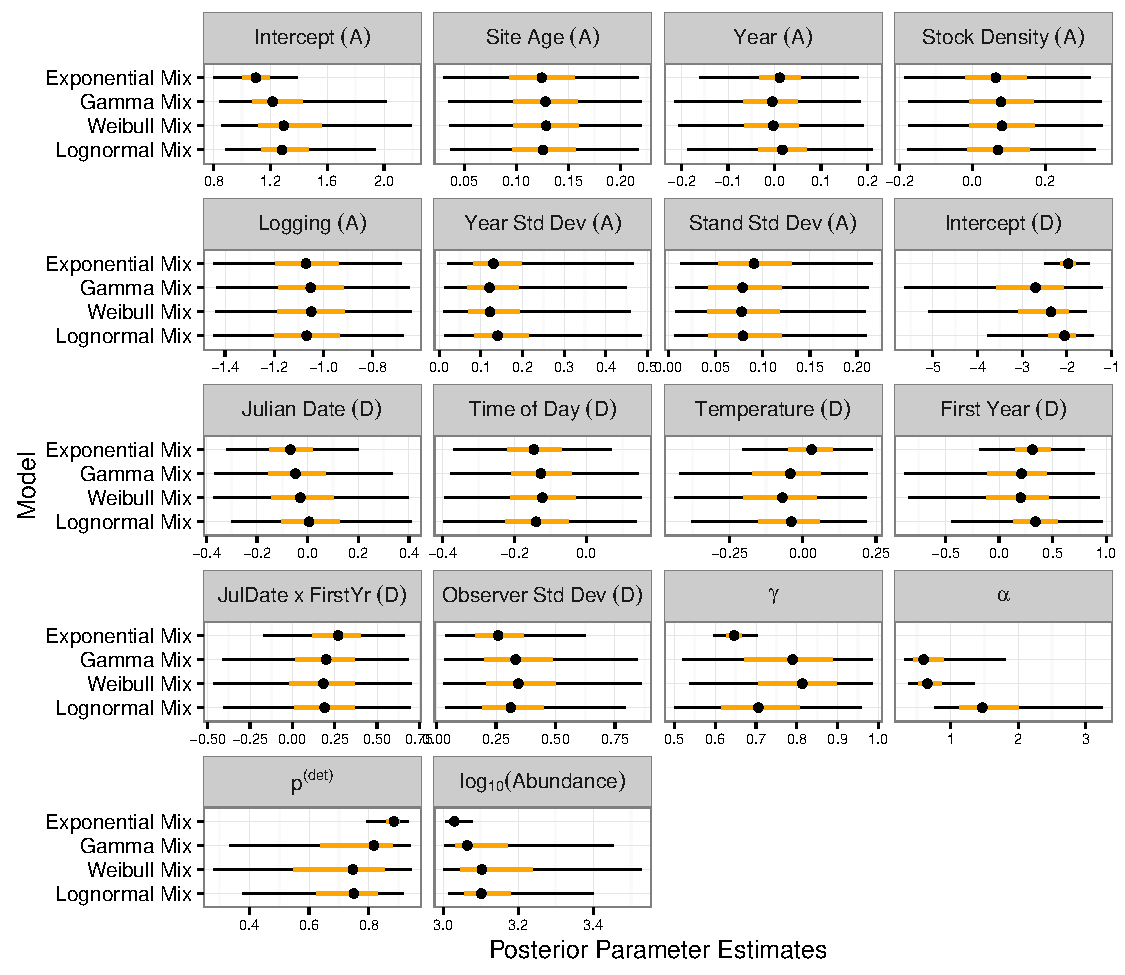
\includegraphics[width=0.95\textwidth]{OVEN/oven_sum/OVEN_Posteriors}
\caption{\label{ovenposteriors} Posterior medians (black dots) with 50\% (wider line) and 95\% (narrowerline) credible intervals for the mixing parameter ($\gamma$), shape parameter ($\alpha$) as well as abundance (A) and detection (D) fixed effects and random effect standard deviations.
Posteriors are also available for the number of uncounted individuals and the overall probability of detection across all sites.}
\end{figure}





\section{Discussion} \label{sec:discuss}

We formulated a model for interval-censored time to detection data that allows for non-constant detection rates.
Our model adopts a time-to-event approach within a hierarchical N-mixture framework, and it allows times to first detection to be modeled according to flexibly defined TTDD families.
Our results show that non-constant TTDDs can return reasonable estimates of detection probabilities across a variety of time-to-detection data patterns, whereas traditional constant-rate TTDDs return biased and overly precise estimates when data deviate from the constant-rate assumption, even when they include a mixture for heterogeneity across groups.  
Because the exponential TTDD is a special case of both gamma and Weibull TTDDs, we can interpret the differences in estimation between models as resulting from the information conveyed by the assumption of constant detection.
%Phrased differently, in the Bayesian context, the exponential model is equivalent to a gamma or Weibull model where the prior for the shape parameter $\alpha$ is defined: Pr($\alpha=1) = 1$; and the differences between the models results from the strength of this prior.
Among the TTDDs modeled in our study, the gamma mixture TTDD gave the most accurate estimates across data distributions, though the Weibull mixture TTDD was comparable for peaked datasets.  

We have additionally demonstrated for non-constant models the utility of using a mixture TTDD formulation.
Inference models with a mixture component are accurate whether the data have a mixture or not, whereas inference models without the mixture are badly biased when the data do feature a mixture.  
Mixture models even outperform non-mixture models when the data are non-mixture and nonpeaked.
%For a discussion of mixtures as heterogeneity, see Pledger 2000, dating all the way back to Otis 1978.

If the estimation of effect parameters and the roles of explanatory variables are the primary interest, then our results suggest that the exact choice of TTDD may not be important.  
Abundance effect estimates are similar regardless of the chosen TTDD.
Detection effect estimates, while conditional on the mixing parameter $\gamma$, are similar across all mixture non-exponential TTDDs.  
These findings may well not hold if the same covariate is modeled in both abundance and detection models \citep{Kery2008}.

\ifdic
In a limited set of situations, posterior predictive checks and DIC can identify when non-mixture or exponential TTDDs inadequately describe the marginal pattern of detections over time.  
But in many situations, neither tool points a clear way to select the correct family of TTDD.  
\fi

If the estimation of abundance is the primary interest, then the choice of TTDD has large consequences, and we may reasonably ask whether removal sampled point-count surveys are adequate for the purpose.  
The strategy behind removal sampling is to use the pattern of detections over time to estimate the proportion of individuals that would be detected if only the observation period lasted longer.  
As such, it is entirely based upon extrapolation and correctly estimating the probability in the tail of the TTDD based on recorded observations.
An assumption of constant detection places constraints on the amount of uncertainty in the extrapolated tail but at the cost of potentially sizable bias.
When we allow for non-constant detection, estimation of the tail probability becomes less certiain.
In theory, estimation of the unsampled tail probability can be improved by conducting longer surveys, but the longer the survey lasts, the greater the risk that individuals enter/depart the study area or are double-counted, which violates the removal sampling assumption of a closed population \citep{LeeMarsden2008, Reidy2011}.  
Without extending the observation period, an alternative to removal sampling is to record complete detection records (all detections for every individual) instead of just the first \citep{Alldredge2007}; however, this may not be feasible in studies like MNFB where many species are observed simultaneously

%With the increasing use of microphone arrays for automated detection, it is tempting to think TTDD models may be valuable for microphone-collected data.  
%This should be the case when variations in detection result solely from organismal behaviors, such as bout singing, or if we wish to model individual random effects in the detection model.  
%However, some explanations for non-constant detection are explicitly related to the observation process --- either effects of the observer on animal behavior or variations in observer effort caused by survey methodology.  
%The assumption of constant detection seems more plausible in studies where observers are absent, though detection heterogeneity may still exist across subgroups of the population.

Versions of time-varying models have been described for trap-based removal sampling and continuous-time capture-recapture.  
Time variation has been modeled through a non-constant hazard function \citep{Schnute1983, HwangChao2002}, a randomly varying detection probability across trapping sessions \citep{WangLoneragan1996}, and constant detection probabilities that vary randomly from individual to individual \citep{Mantyniemi2005, Laplanche2010}.
Most of these approaches resulted marginally in a decreasing (nonpeaked) detection function over time.  
Their results generally echo what we have presented here.  
\citet{Schnute1983} found that the equivalent of a mixture exponential adequately described their data.
\citet{WangLoneragan1996}, \citet{HwangChao2002}, and \citet{Mantyniemi2005} all found constant-detection models to be flawed, producing underestimates of abundance and too-narrow error estimates; these resulted in inadequate coverage and also overstatement of effect significance.  
%Schnute: allowed time-varying detection which collapsed to a mixture model
%Wang and Lonergan: \pi_s ~ beta for each interval at a site... not particularly applicable in an avian framework (with arbitrarily partitioned), except perhaps for bout singing?
%- didn't have group heterogeneity
%- constant models are overly precise (factor of 3)
%Mantyniemi: individual-level variation in \pi_s ~ beta
%- large number of trapping sessions required to overwhelm prior on variance (8-12)
%- could also be viewed in terms of percent of total caught
%- constant detection model badly biased
%- constant detection model made indexing unreliable, since pairwise differences could be magnified
%Laplanche: model selection with site-level abundance variation, site-level catchability variation, and individual-level catchability variation.
%- only the abundance proved significant
%Hwang and Chao: time-varying capture-recapture
%- use a nonpeaked hazard function
%- again, the constant model underestimates abundance, with coverage between 0-6\% for 95\% credible intervals (even allowing for covariate-based individual effects and behavioral responses).

Point-count survey data often include the recorded distance between observer and detected organism.
Because our focus has been on modeling variations in detection rates during the survey period, we have not incorporated distance into our model.
Consequently, our application of a TTDD represents an averaging across distance classes, which induces systematic bias in estimates of abundance \citep{EffordDawson2009, Solymos2013}.  
To be consistent with the continuous time-to-event approach, distance can be incorporated into the detection model as an event-level modifier as is done in \citeauthor{borchers2015}.  
This approach is distinct from earlier integrations of removal- and distance sampling, where distance has been treated as an interval-/survey-level modifier \citep{Farnsworth2005, Amundson2014}.
The differences between these implementations may impact estimates of detection and abundance, especially in the presence of behavioral heterogeneity in availability rates across subgroups of the study population.  
This is an area of ongoing exploration.
%Our adoption of a time-heterogeneous continuous time-to-detection approach in our model mirrors continuous time work in mark-and-recapture \citep{HwangChao2002, FarcomeniScacciatelli2013, Borchers2014}.

%Examples of the interval-censored approach.
%\citep{Farnsworth2002, Royle2004Generalized, Farnsworth2005, Alldredge2007, EffordDawson2009, Etterson2009, Reidy2011, Solymos2013, Amundson2014, Reidy2016}.

%In a distance-sampling context, the probability of detection for any individual is framed as the joint probability of two independent detection events: (i) availability for detection, which occurs during an observation period with probability $P_a$, and (ii) detection of the available individual by an observer, $P_b$, also known as perceptibility \citep{Williams2002, Kery2008, Nichols2009}... citations too numerous to enumerate.
%In avian point-counts, because the overwhelming majority of detections are auditory, $P_a$ is understood to be the probability that a bird vocalizes during the observation period.  
%Meanwhile, perceptibility is treated as a function of distance $d$: $P_b = g(d)$, with nearby available individuals being detected with higher probability than distant individuals.  
%The probability of detection is thus formulated as availability times perceptibility: $\pdet = P_aP_b$.  
%However, our analysis makes possible a different strategy that is more consistent with a time-to-event conceptualization of the problem.  
%Rather than define availability and perceptibility as independent detection events over the course of the observation period, we can define them at the event level.  
%In terms of the model we have presented in this paper, this is equivalent to redefining the time-to-detection hazard function, $h_{sq}(t)$ --- which is now a function of the distance to individual $q$ --- as the product of the time-to-availability hazard function $h_{s}^A(t)$ and the perceptibility function $g(d_q)$.  
%So, $h_{sq}(t) = g(d_q) h_{s}^A(t)$.  
%From standard survival analysis results, $p_{sq}^{(det)} = 1 - \exp\left(-g(d_q)\int\limits_0^{C_I} h_{s}^A(u)du\right) = 1 - \left[1 - F_T^A(C_I|\varphi_s, \boldsymbol{\theta}) \right]^{g(d_q)}$.
%In short, the time-to-event conceptualization frames perceptibility as a rate-of-availability multiplier rather than as a probability-of-availability multiplier.  
%In a context where rates of availability are allowed to vary from individual to individual, this makes an intuitive sense --- a bird that sings twenty times during the observation period should have its overall detection probability discounted much less than a bird at the same distance which only sings once.  

% Skeptics of removal sampling: Johnson08, EffordDawson09, Reidy11

We recommend that time-heterogeneous detection rates be explicitly modeled in analyses involving removal-sampled point-count survey data where estimation of detection probability or abundance is a primary objective.  
The assumption of constant detection, while computationally simple and reasonable as a null model, proves to be rather informative and can result in pronounced bias.  
Meanwhile, the causes of non-constant detection -- i.e., observer effects on behavior and systematic variations in observer effort -- are both plausible and not trivially discounted.  
It would be nice if the data itself could inform us whether constant detection is a reasonable assumption; however, our preliminary efforts to diagnose this assumption using deviance information criterion (DIC) and posterior predictive check statistics have led to weak and sometimes erroneous findings.
Development of such a diagnostic tool would be useful, but given the limitations of first time-to-detection data, we are not confident a reliable tool could be easily developed.  
We believe that more informative data collection, such as complete time-to-detection histories and microphone arrays, offer more effective tools for time-to-event modeling going forward.

% \adam{Topics I have omitted from the Discussion (which reflects my own judgment, but you may disagree):
% \begin{enumerate}
% \item Selection of priors (especially for intercepts; also, the possibility of a spike-and-slab for $\alpha$)
% % Note: now that I've seen van Dishoeck and Mantyniemi, perhaps I should worry about informativeness in priors.}
% \item Values for $\pdet$ used in simulations
% \end{enumerate}
% }





\bibliography{masterbib}
\bibliographystyle{biom}

\end{document}
